% \documentclass[]{amsbook}
\documentclass[12]{article}

% \input MyMacros.tex

% \usepackage[pdftex]{graphicx}
\usepackage{dcolumn}% Align table columns on decimal point
\usepackage{bm}% bold math
\usepackage{verbatim} % this is needed for \begin{comment} ... \end{comment}
\usepackage{lscape} % this is needed for occasional landscape figures
\usepackage{amsmath}
% \usepackage{appendix}
%\usepackage{subfigure}
%\usepackage{epsfig}
\usepackage{amsfonts}
\usepackage{multicol}
\usepackage{graphicx}
\usepackage{caption}
\usepackage[margin=1.1in, top=1.1in, bottom=1.1in]{geometry}

% \textwidth 550pt
% \textheight 500pt
% \hoffset -3.5cm
\def\betabold{{\pmb{$\beta$}}}

\setcounter{tocdepth}{3}
%
\begin{document}

\date{January, 2013}

% \voffset=1.5
\title{
\centerline{}
\centerline{}
\centerline{}
UAL/ETEAPOT Proton EDM Benchmark Report IV: \\ 
Comparison of ETEAPOT, Linearized Transfer Matrix, \\
and Runge-Kutta Proton EDM Lattice Results (DRAFT)
}
\author{R.M.. Talman and J.D. Talman
}

\maketitle

% \tableofcontents

\begin{abstract}
Valeri Lebedev's new, all-electric proton EDM lattice, 
(here referred to as {\tt E\_ValLeb2-sl4-RF.sxf}), which is
strong-focusing radially, weak-focusing vertically, is 
treated as the most up-to-date lattice for purposes of 
benchmark comparison of various lattice calculation codes. 
For transverse optics the agreement among three independent 
analyses, two based on the Wollnik transfer matrix formalism, 
one using the TEAPOT lattice simulation code, is excellent. 
Plots and tables bear this out.
The understanding of longitudinal dynamics, though still murky, 
is clearer than previously. A crude comparison between ETEAPOT 
and Runge-Kutta analysis of longitudinal dynamics in a
previous benchmark lattice {\tt E\_BM\_Z-RF.sxf} is given. 
Factors making such comparisons delicate are discussed. 
The importance of proving beam capture into stable longitudinal 
buckets is emphasized. In fact, unlike {\tt E\_BM\_Z-RF.sxf},
attempts to achieve stable capture into the 
{\tt E\_ValLeb2-sl4-RF.sxf} lattice have failed so far.
It is not known at present whether this is a property of the
lattice, which would be surprising, or a bug in ETEAPOT.
\end{abstract}
%

\clearpage

\section{Parameters of Benchmark Proton EDM Lattices}
This section concentrates on treating the proton EDM lattice
proposed by Valeri Lebedev\cite{ValLeb2} as the most up-to-date 
``benchmark comparison lattice'', following  previous benchmark 
comparisons\cite{Benchmark-I}\cite{Benchmark-II}\cite{Benchmark-III}\cite{YKS-tracking}.
This lattice (in \emph{standard exchange format} form it is {\tt ValLeb2-sl4.sxf})
has strong horizontal focusing and weak vertical focusing. 

Transverse Twiss parameters have been calculated from linearized transfer matrices
in two different ways, one described in this report, and referred to as R.M.T., 
and one from the initial Lebedev report\cite{ValLeb2} and referred to as V.L. 
Both of these analyses are based on the Wollnik\cite{Wollnik} linearized transfer 
matrix formalism. As such, they are independent only as regards lattice details, 
element slicing, and interpretation of the formalism. The third analysis, based
on ETEAPOT is here referred to as J.D.T. The ETEAPOT approach is to perform 
exact tracking in an approximate lattice, and to reconstruct the Twiss parameters
by numerical post-processing the results from tracking
a standard bunch of 21 small amplitude particles.
Being based on entirely different formalisms, the comparison of ETEAPOT and
Wollnik-based results can provide a stringent test of our understanding of 
the proposed proton EDM lattice.

Comparisons of transverse lattice parameters are given in Table~\ref{tbl:TransverseParams}.
The R.M.T and J.D.T. analyses are based on lattice file {\tt ValLeb2-sl4.sxf} which
has been reconstructed from the original Lebedev\cite{ValLeb2} report. The lattice
is simple enough, and the Lebedev report careful and thorough enough, that this
reconstruction could be performed with little ambiguity. The only significant
uncertainty was that only the ratio of quadrupole fields GDD/GFF, rather than
the absolute quad strengths (i.e. inverse focal lengths) is given in the report 
\cite{ValLeb2}. The tunes $Q_x$ and $Q_y$ are given, however, and, from these, 
the absolute (half-)quad strengths $qFh$ and $qDh$ have been determined.
%
\begin{table}[h]
\caption{\label{tbl:TransverseParams}Transverse lattice parameters of the proton EDM 
lattice proposed by Valeri Lebedev\cite {Benchmark-I}, as evaluated in three independent 
ways. This lattice (here referred to as {\tt ValLeb2-sl4.sxf}) can serve as a new
(most realistic so far) benchmark lattice. 
} 
\medskip
\centering
\begin{tabular}{|c|c|c|c|c|c|c|c|c|c|c|c|}           \hline
Analysis   & author & half-quad & quad ratio & horz. & vert. &     max.     &     min.      &     max.      &     min.      \\
 method    &        &  strength & GDD/GFF or & tune  & tune  &    horz.     &     horz.     &    vert.      &    vert.      \\ 
           &        &  $qFh$    & $qDh/qFh$  & $Q_x$ & $Q_y$ &   $\beta_x$   &   $\beta_x$   &   $\beta_y$   & $\beta_y$     \\ \hline
           &        &   1/m     &            &       &       &       m       &      m        &      m        &      m        \\ \hline
linear tr.mat. &  V.L.  & -0.0307   &  -0.802    & 2.32  & 0.31  &      29.1     & $\approx16$   &    204        &  $\approx118$ \\     
linear tr.mat. & R.M.T. & -0.0307   &  -0.765    & 2.32  & 0.315 &      29.2     &    15.4       &   201.8       &   114.0       \\ 
ETEAPOT    & J.D.T. & -0.0307   &  -0.765    & 2.31  & 0.325 &      29.2     &    15.4       &    196        &   110.8       \\  
\hline
\end{tabular}
\end{table}
%

In the {\tt ValLeb2-sl4.sxf} latice description file, the ``{\tt -sl4}'' indicates
that the bend elements have been artificially sliced by a factor of four, from
about 9 meters to about 2.25 meters. This has been done both for making the
physical construction more realistic, and to relieve the burden on ETEAPOT tracking
over such long elements. As it happens, ETEAPOT automatically performs a further
splitting of a factor of two, to make lattice parameters available at element
centers. Also ETEAPOT can perform further splitting in order to represent bend
elements having field indices other than $m=0$ (which corresponds to ``cylindrical''
bent-planar, parallel electrodes). However for the present study we fix $m=0$.

Table~\ref{tbl:TransverseParams} shows excellent agreement among the three approaches.
With $qFh$ constrained to be identical for all studies, the only discrepancy is
in the ratio $qFh/qDh$ which differs at most by 4.6\%, from -0.802 to -0.765.
A discrepancy at least this large can be expected from the fundamental ambiguity
in the treatment of electric elements, especially in the comparison between
ETEAPOT and Wollnik approaches.  As it happens there is essentially no
difference in the treatments based on the identical lattice description file, 
and the entire discrepancy is between V.L. and R.M.T. implementations of 
the Wollik approach on slightly different lattices. In any case all
comparisons are sufficiently excellent that there can be no doubt the the
transverse lattice performance will be essentially just as Lebedev has 
first stated. One must keep in mind, however, that the lattice with 
unbalanced focusing is quite ``highly strung''.  For example, a 1\%
change in the $qDh$ focal length reduces $Q_y$ from 0.3 to 0.0 (where
the lattice becomes unstable). 

R.M.T. linear transfer matrix Twiss functions are compared to J.D.T. ETEAPOT
Twiss functions in Figures~\ref{WollnikVsETEAPOT-x} and \ref{WollnikVsETEAPOT-y}. 
V.L. linear transfer matrix Twiss functions are compared to ETEAPOT
Twiss functions in Figures~\ref{fig:ValLeb2Twiss} and \ref{ETEAPOT-twiss}. 
There is essentially perfect agreement in all cases.

\begin{figure}[h]
\begin{minipage}{0.5\linewidth}
\centering
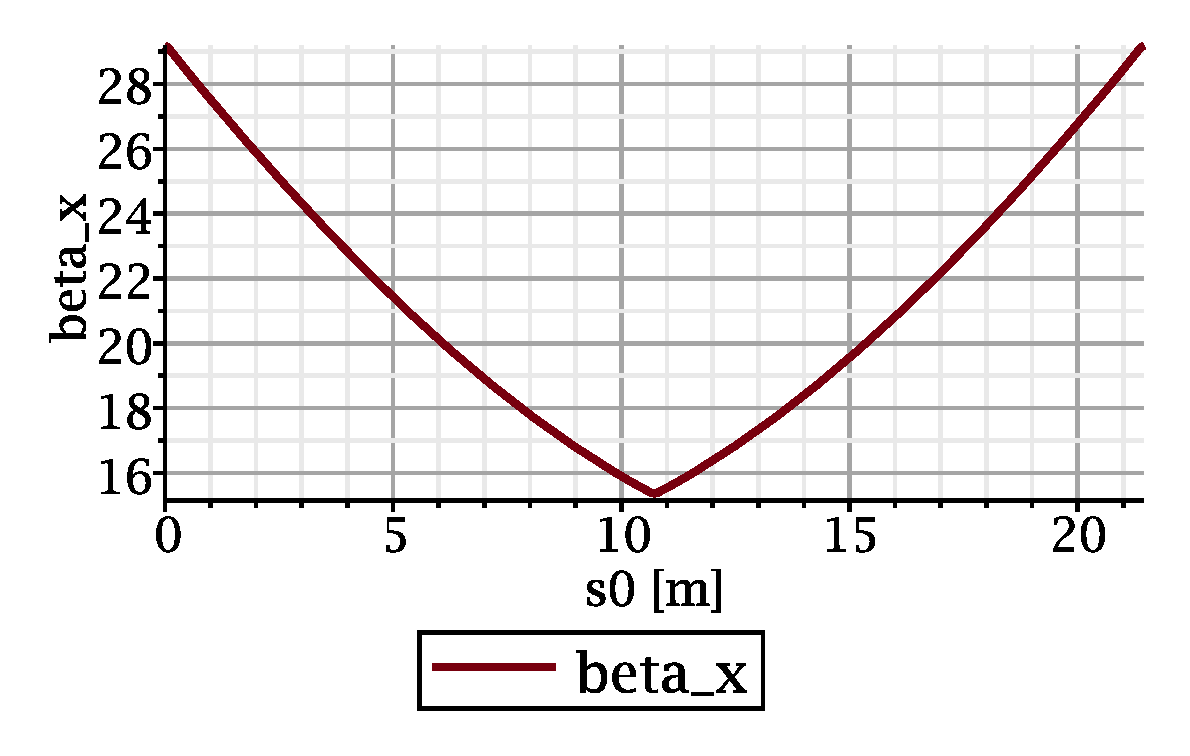
\includegraphics[scale=0.4]{betax_1cell.eps}
\end{minipage}
\begin{minipage}{0.5\linewidth}
\centering
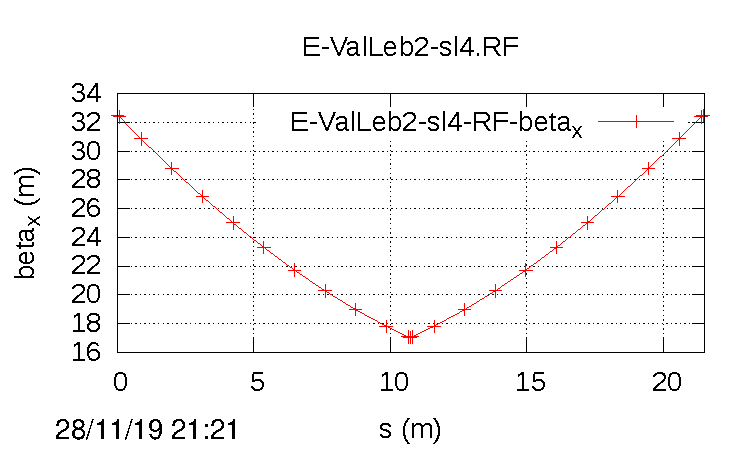
\includegraphics[scale=0.7]{E-ValLeb2-sl4-RF-betax.pdf}
\end{minipage}
\caption{\label{WollnikVsETEAPOT-x}Proton EDM Lattice $\beta_x$ functions as determined by
linear transfer matrix formalism, on the left, and by ETEAPOT,
on the right.}
\end{figure}

\begin{figure}[h]
\begin{minipage}{0.5\linewidth}
\centering
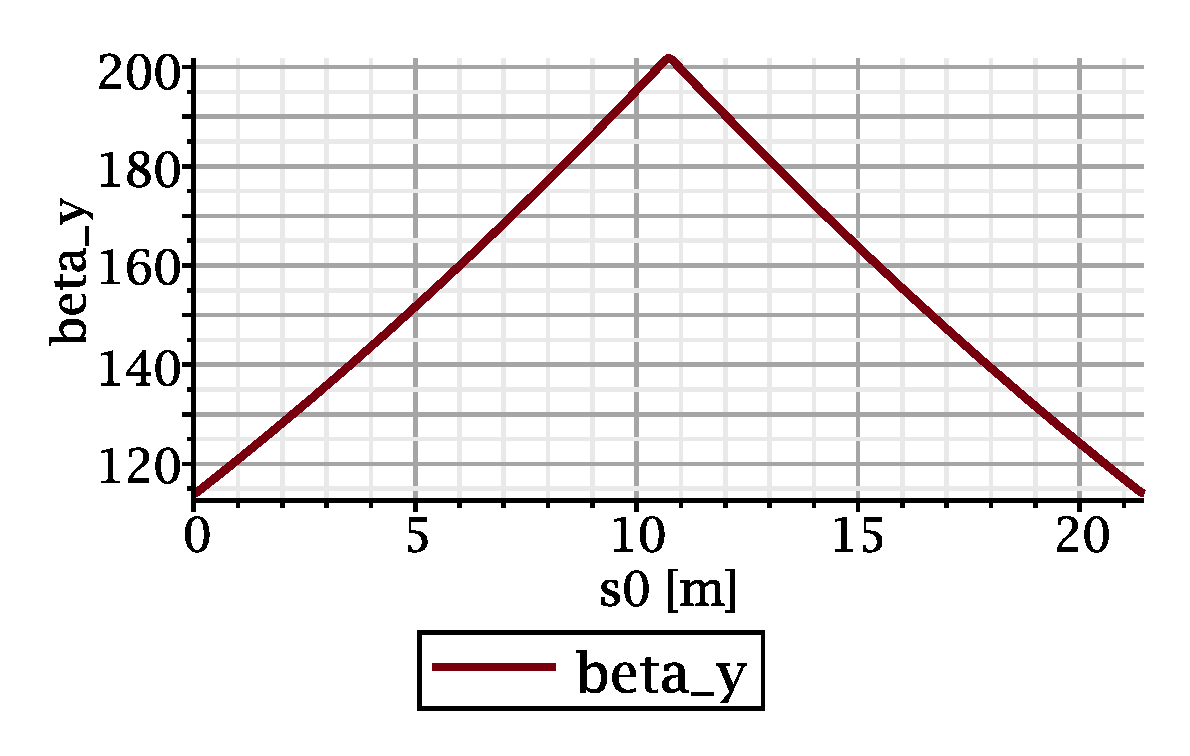
\includegraphics[scale=0.4]{betay_1cell.eps}
\end{minipage}
\begin{minipage}{0.5\linewidth}
\centering
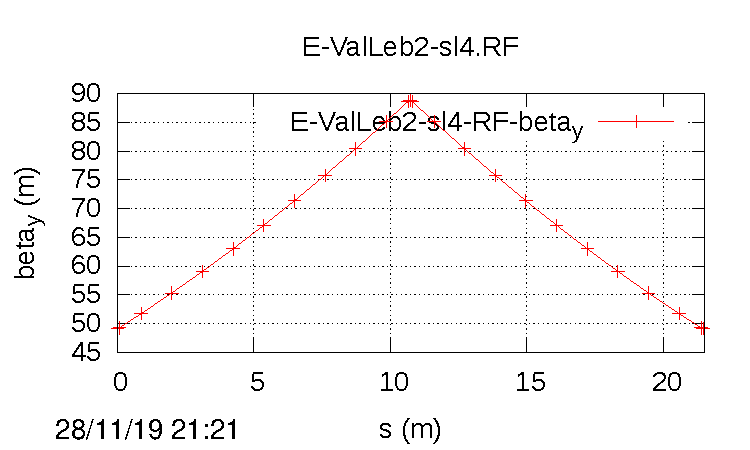
\includegraphics[scale=0.7]{E-ValLeb2-sl4-RF-betay.pdf}
\end{minipage}
\caption{\label{WollnikVsETEAPOT-y}Proton EDM Lattice $\beta_y$ functions as determined by
MAPLE linear transfer matrix formalism, on the left, and by ETEAPOT, on the right.}
\end{figure}

\clearpage

Figure~\ref{fig:ValLeb2Twiss}, copied directly from the original Lebedev report,
gives his beta functions and dispersions. For comparison the ETEAPOT plots
are repeated in Figure~\ref{ETEAPOT-twiss}. Again the agreement is excellent.

\begin{figure}[h]
\centering
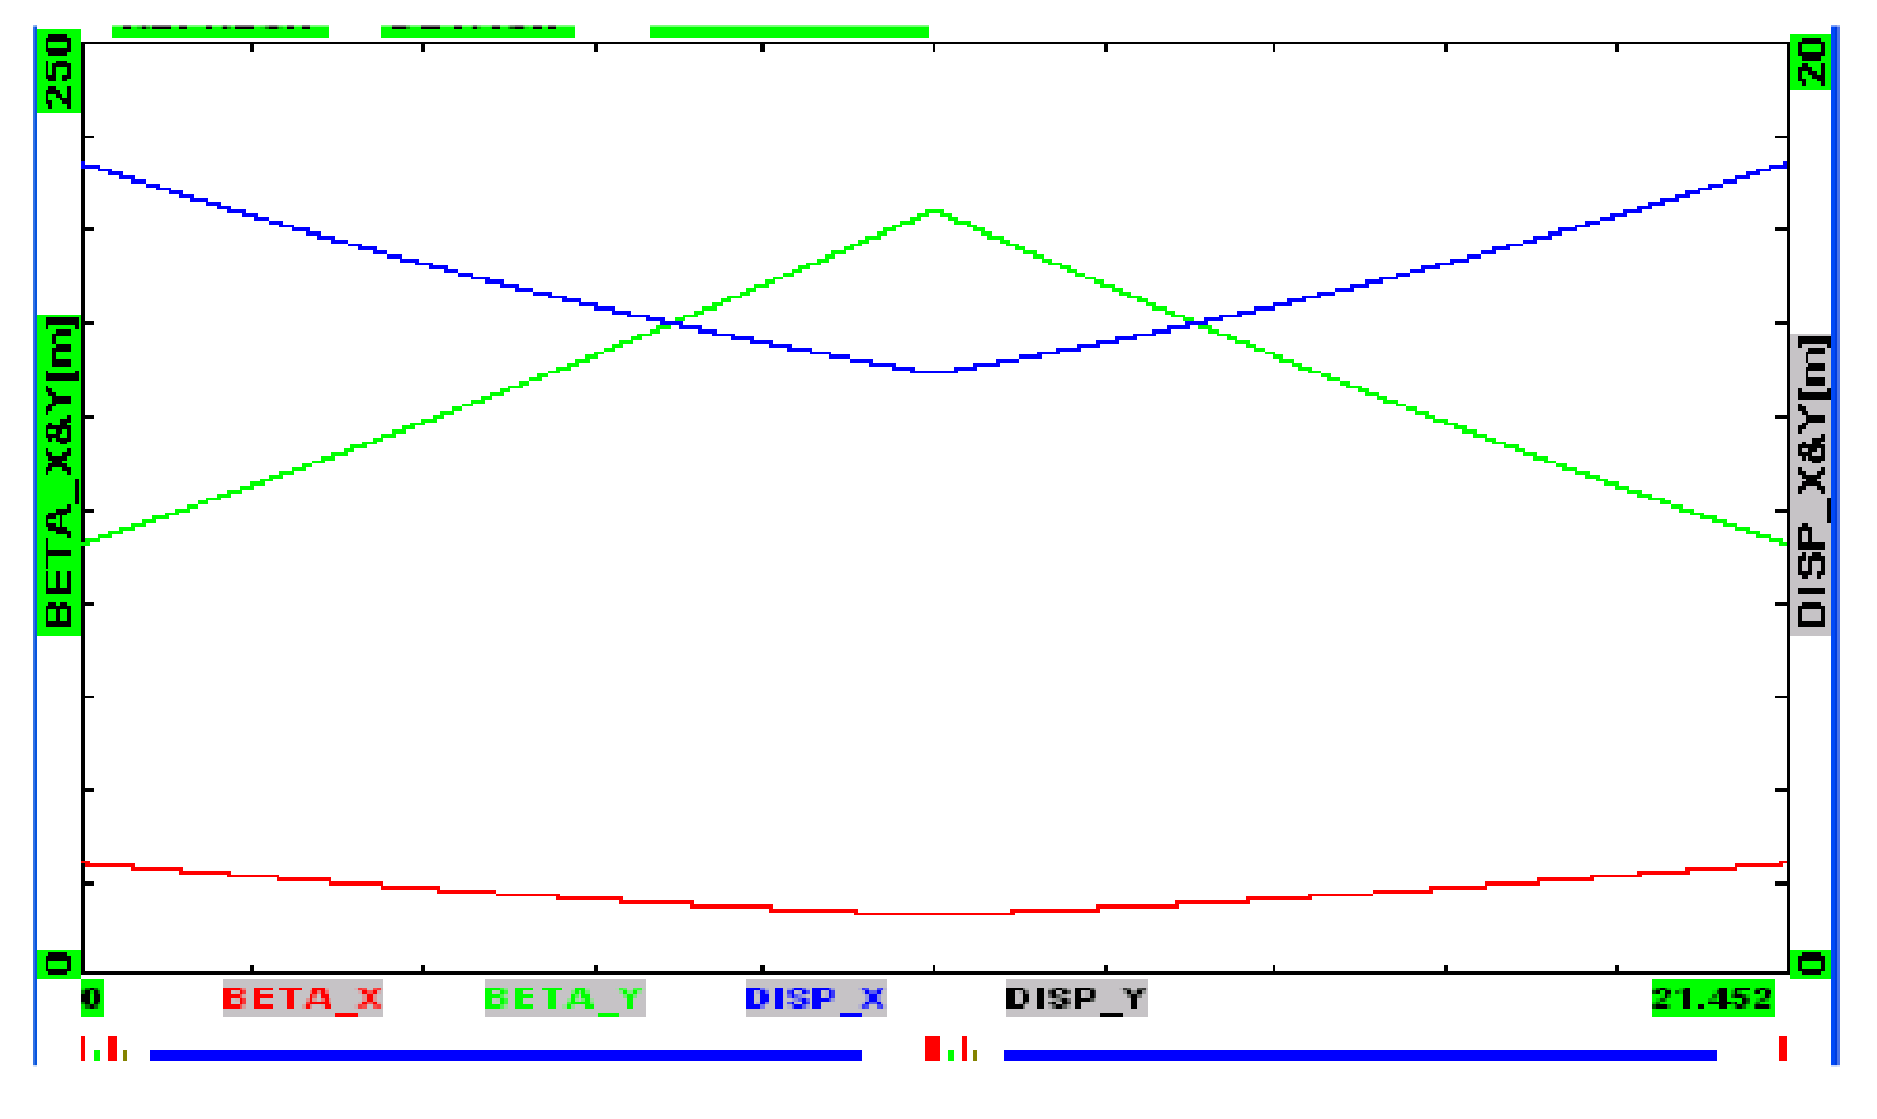
\includegraphics[scale=0.4]{ValLeb2-twiss.pdf}
\caption{\label{fig:ValLeb2Twiss}Proton EDM Lattice $\beta$ functions as determined by
Valeri Lebedev\cite{ValLeb2}. Also shown is the dispersion function.}
\end{figure}

\begin{figure}[h]
\centering
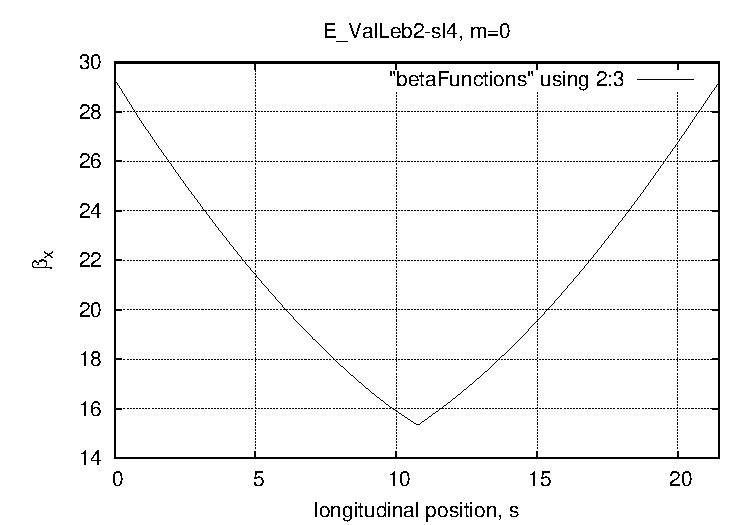
\includegraphics[scale=0.55]{ETEAPOT_ValLeb2-sl4betax.pdf}
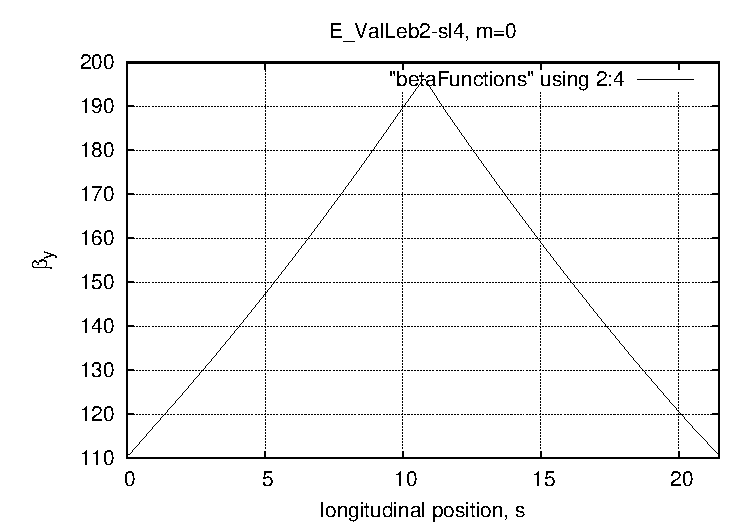
\includegraphics[scale=0.55]{ETEAPOT_ValLeb2-sl4betay.pdf}
\caption{\label{ETEAPOT-twiss}Proton EDM Lattice $\beta$ functions as determined by
ETEAPOT. Ambiguity in the definition of ``dispersion'' complicates comparison
with the Lebedev dispersion. Though not yet completed, there is every reason to
expect similarly good agreement.}
\end{figure}

\clearpage

\section{Comparison of Longitudinal Dynamics}
Though transverse dynamics in all-electric proton EDM rings is now 
completely under control, the same cannot be said for longitudinal
dynamics.  From now on it will be important, appropriate, and possible, 
to concentrate more on longitudinal dynamics.  

Previous benchmark comparisions of results
of ETEAPOT and Runge-Kutta tracking showed 
seemingly contradictory results. For example ETEAPOT tracking\cite{Benchmark-III} 
showed long term instability limiting the dynamic aperture
to be about an order of magnitude less than given by Runge-Kutta 
tracking\cite{YKS-tracking}. We have now
realized that this inconsistency may be partially understood in terms of
the vastly disparate peak RF voltages that were being assumed for the
two studies. In both cases harmonic number $h=100$ was assumed, but 
the largest peak RF voltage in the ETEAPOT study was 5\,KV, whereas, 
in the Runge-Kutta study the peak voltage was 1\,MV. 
This factor of 200 difference can certainly be expected to affect the
comparison. Extending the range of RF voltages in the ETEAPOT study 
to 0.1\,MV (above which instability results) one obtains the comparison 
shown in Figure~\ref{fig:YKS-ETEAPOT-compare}. This is not intended
as evidence of ``agreement'' between the results; rather it is intended 
as a beginning on the route to eventual, more controlled, comparison. 
Complications in performing such comparisons are discussed next.

\begin{figure}[h]
\centering
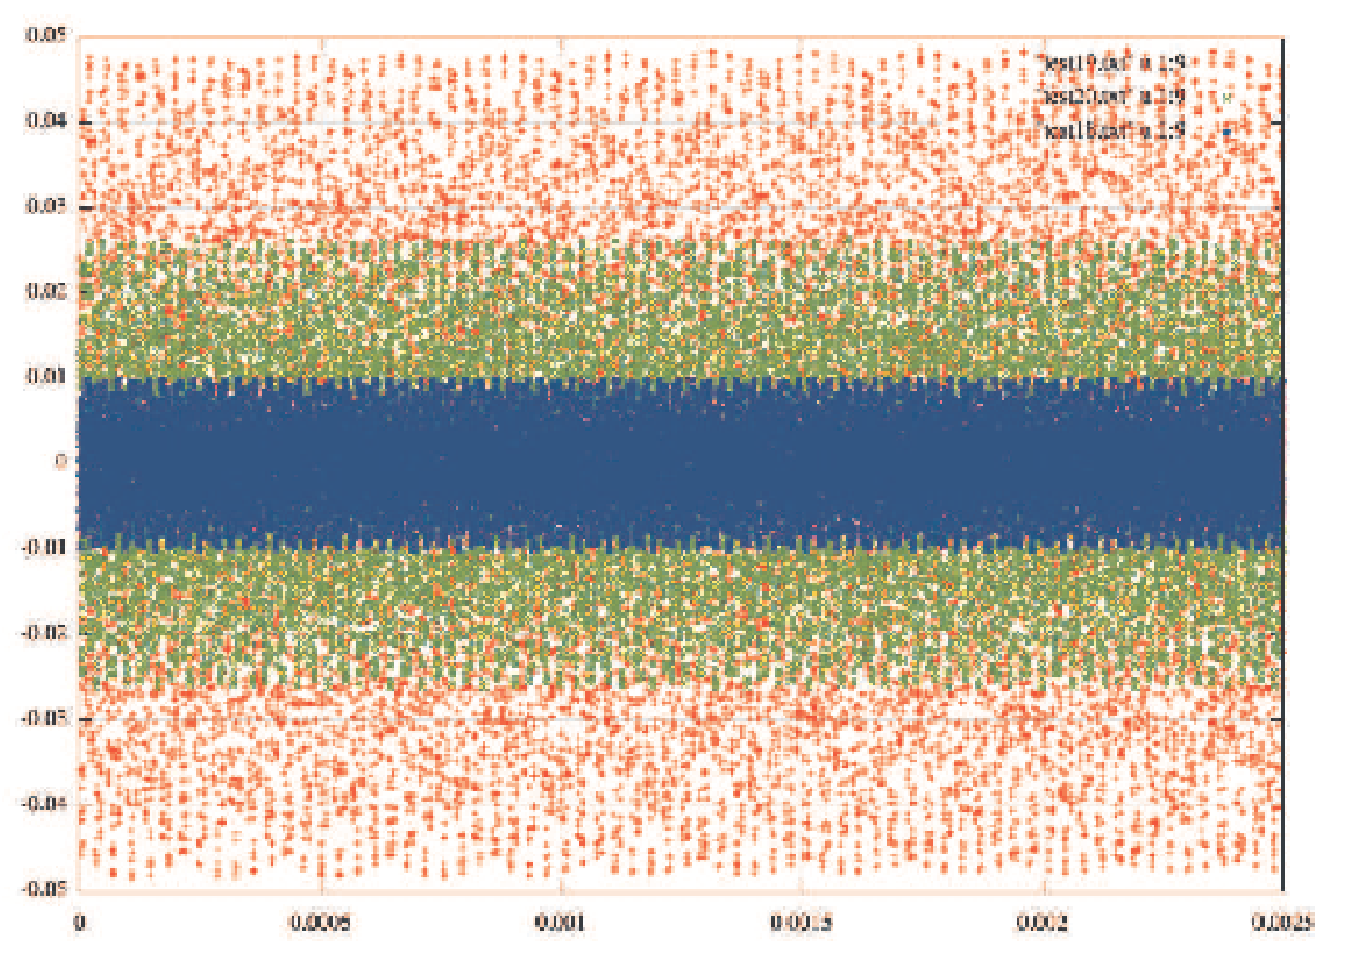
\includegraphics[scale=0.35]{Yannis-RungeKutta.pdf}
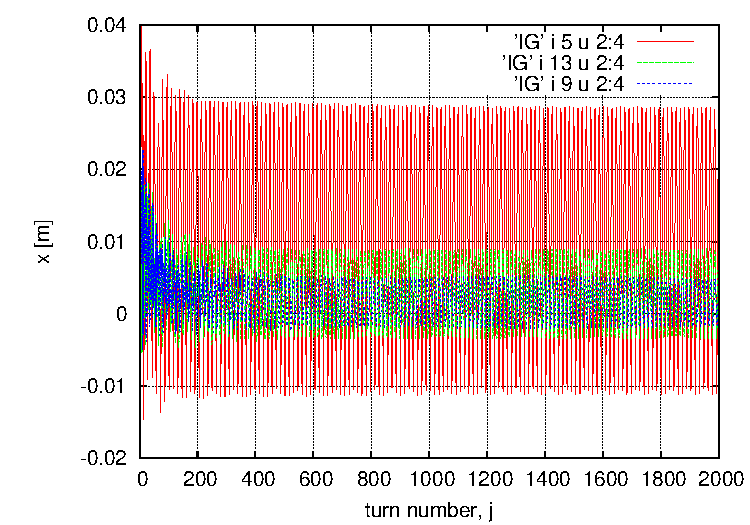
\includegraphics[scale=0.6]{CheckYKS-Fig18.pdf}
\caption{\label{fig:YKS-ETEAPOT-compare}Comparison of
(Figure 18 of reference\cite{YKS-tracking}) 
Runge-Kutta tracking (on the left) with ETEAPOT tracking
(on the right). In both cases the three traces correspond
to initial $x$-amplitudes of -1\,cm (blue), 0 (green), and 
+1\,cm (red), all with $\Delta p/p=2\times10^{-4}$. The x-ranges 
of both plots are about the same. For the Runge-Kutta plot
the RF voltage was 1\,MV. For the
ETEAPOT plot the RF voltage was 0.1\,MV
(approximately the highest voltage for which the
particles could be captured into stable buckets). This
comparison is discussed (and qualified) further in the text.
}
\end{figure}
Though it has been stated that the same lattice (namely {\tt E\_BM\_Z-RF.sxf})
has been used in the ETEAPOT/Runge-Kutta comparison, this is only approximately
true, especially as regards the (weak) vertical focusing needed to preserve
vertical stability. Furthermore the $m$-values are slightly different.
These blemishes are not expected to be significant.

The ETEAPOT/Runge-Kutta comparison in Figure~\ref{fig:YKS-ETEAPOT-compare}
is as close as it is only because various empirical adjustments
(for example resolving ambiguous lattice details to make the plots look
more similar) have been made.
Furthermore, though the three ETEAPOT initial displacements are displaced from
each other by 1\,cm, they have been allowed to shift together radially to compensate
for a possible shift of the fixed point about which linearized expansion
is valid. (Allowing this freedom can only be justified as an interim procedure.) 
Even so, casual observation shows significant disagreements 
remain, especially the up-down asymmetry on the right but not on the left,
and different amplitudes. One hint of difficulty, shared by both plots, 
is that the +1\,cm and -1\,cm traces are not the same, except for sign,
which is what one might have expected. 

While it has been easy to specify transverse-sensitive lattice
conditions unambiguously it is harder to specify longitudinal
conditions. There is ambiguity as to whether the beam is specified 
inside or outside electric field regions; the change in kinetic
energy in passing from inside to outside affects this specification.
It is also important to specify where in the ring the RF cavity is
situated, as beam capture depends on this. If the RF cavity is
at the beginning or end of the lattice (as is convenient for such studies) 
it is essential to know whether the beam is injected just before or
just after the RF. More generally, the specification of longitudinal
performance depends on the full, six-dimensions in phase space,
of the initial bunch distribution.

The fine grain structure of the ETEAPOT and Runge-Kutta plots in
Figure~\ref{fig:YKS-ETEAPOT-compare} are similar. By counting red peaks one
finds the ``synchrotron tune'' $Q_s$ of this granularity to be 
$Q_s=14.2/200=0.071$ for the ETEAPOT plot. (Though it is not possible to infer 
it from the fuzzy plot) this is the same for all three traces; 
see Figure~\ref{fig:RK-compare-longit}. For the outermost
(red) Runge-Kutta plot there are 14 periods in 0.0005\,s, which corresponds to
357 turns. This yields $Q_s=14/357=0.039$. Again, the blue and green peaks
are too fuzzy to be counted in the figure as reproduced here. But the
plots in the original report\cite{YKS-tracking} are clearer, and there
seem to be 15.5 green peaks over the same interval that there are 14
red peaks. If true, it would imply the red and green particles have not
been captured in the same bucket. This should be checked. 

To illustrate these issues further, Figure~\ref{fig:RK-compare-longit}
shows the longitudinal phase space evolution corresponding 
to the ETEAPOT data on the right in 
Figure~\ref{fig:YKS-ETEAPOT-compare}. The most essential aspect of
this figure is that the particles are limited to the longitudinal
range from -0.8\,m to +0.8\,m. In other words, the particles have
been captured into a stable bucket. This limitation, specific to capture
into a stable bucket, cannot be inferred from 
Figure~\ref{fig:YKS-ETEAPOT-compare}. 

From the comparison of 
Figures~\ref{fig:YKS-ETEAPOT-compare} and \ref{fig:RK-compare-longit}
one sees also that the 
distribution in transverse amplitude $x$ is strongly correlated
with the range in energy spread $\Delta E/p_oc$. When the
three particles were injected (from zero electric potential outside
bend elements) their kinetic energies were the 
same but, inside electric elements, their kinetic energies have become
different, both because of the different potentials they had to
surmount on entry, and because of the different energies imparted 
by the RF.  
\begin{figure}[h]
\centering
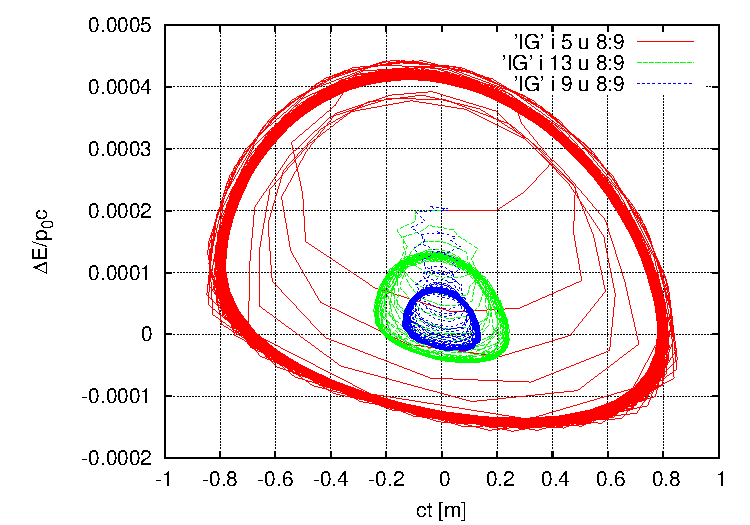
\includegraphics[scale=0.6]{CheckYKS-Fig18-longit.pdf}
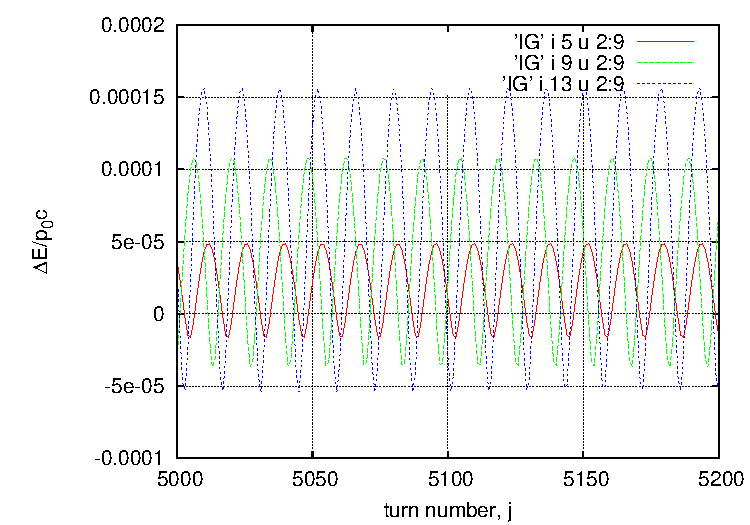
\includegraphics[scale=0.6]{CheckYKS-synchronized-q.pdf}
\caption{\label{fig:RK-compare-longit}Longitudinal phase 
space plots corresponding to the ETEAPOT data on the 
right in Figure~\ref{fig:YKS-ETEAPOT-compare}. The figure
on the right checks that the three traces are exactly
synchronized, as is required for the particles to be in
the same stable bucket.}
\end{figure}

Comparisons of longitudinal dynamics will eventually require
the comparison of entire beam bunches, with realistic spreads
in all phase space dimensions. A small step in this direction
is indicated in Figure~\ref{fig:Centroid}. 

\begin{figure}[h]
\centering
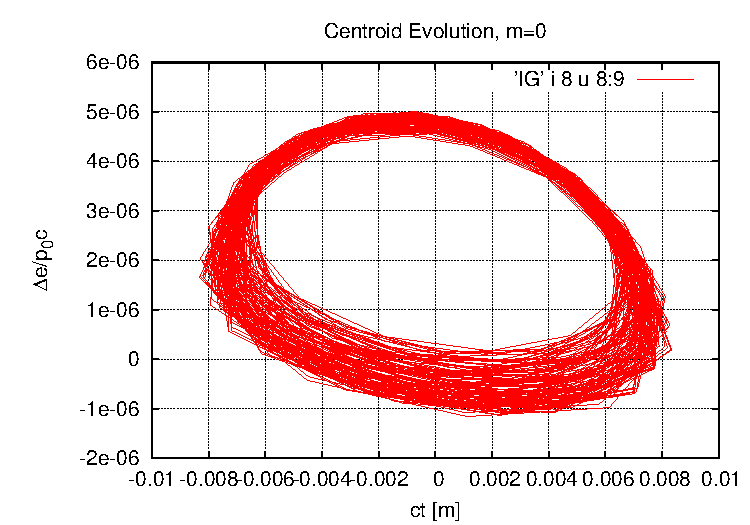
\includegraphics[scale=0.41]{SingleParticleTrack-longit.pdf}
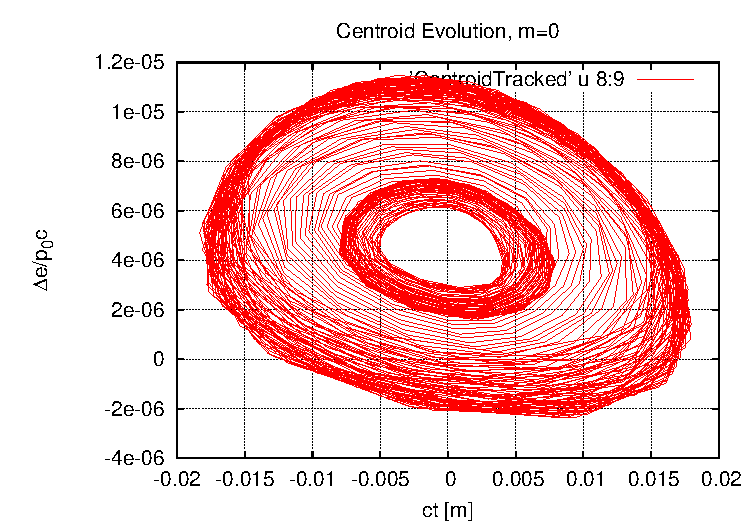
\includegraphics[scale=0.41]{CentroidTrack-longit.pdf}
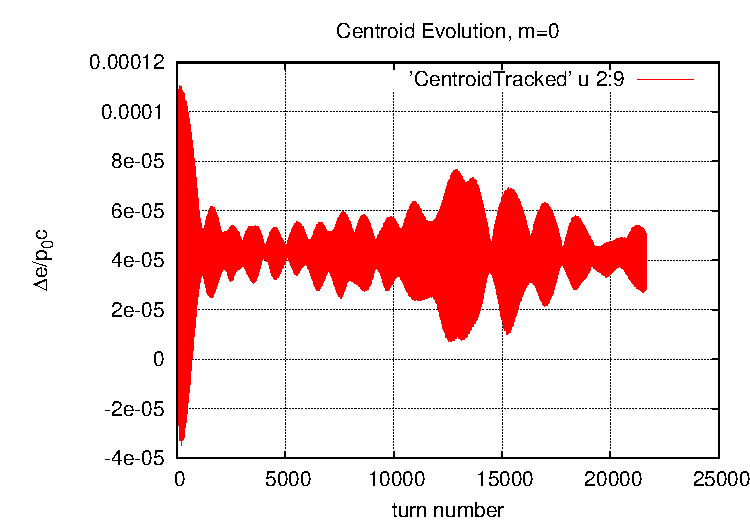
\includegraphics[scale=0.41]{CentroidTrack-mom.pdf}
\caption{\label{fig:Centroid}Longitudinal phase space plots, for
a single particle on the left, and for the centroid of a bunch
of 21 particles in the middle, both for 2000 turns. On the right 
the transverse momentum is plotted for 21500 turns.} 
\end{figure}
The figure is based on 
the longitudinal evolution for 2000 turns of a bunch of 21 particles
initially distributed on-momentum, with zero momentum spread,
and zero angular spread, but uniformly distributed 
radially on the range $-5\,{\rm mm}<x<5\,{\rm mm}$.
The trace on the left is that of a single particle; its
amplitude is more-or-less constant. The trace in the middle is 
that of the centroid of all 21 particles. Its lack of constancy
is due to decoherence, followed by partial recoherence, of
the particles of different amplitude. The figure on the right
shows the centroid momentum plotted for about ten times as many
turns.  Though any one particle executes constant betatron plus
synchrotron oscillations, the centroid drifts quasi-randomly
due to the accidental coherence and decoherence of 21 
particles. (With a real beam of $10^{10}$ particles this fluttery
variation would be negligible.)

As mentioned in the abstract, attempts to achieve stable capture 
into the {\tt E\_ValLeb2-sl4-RF.sxf} lattice have failed so far.
This has not been for want of trying. Hundreds of, admittedly disorganized, 
attempts, including many with the wrong RF frequency, and/or the wrong
RF phase, have been made without success so far. In any case this curious
result is not understood at present.

\begin{thebibliography}{99}
\bibitem{ValLeb2}
V. Lebedev, \emph{Prospects of Strong Horizontal Focusing Electric Ring:
Advantages, Disadvantages,} Storage Ring EDM
Collaboration Meeting, December 9-10, 2013 

\bibitem{Benchmark-I}
J.D. Talman and R.M. Talman, \emph{ UAL/ETEAPOT Results 
(Augmented) for Proton EDM Benchmark Lattices,} BNL internal
report, April 29, 2012

\bibitem{Benchmark-II}
J.D. Talman and R.M. Talman, \emph{ UAL/ETEAPOT Proton EDM 
Benchmark Comparisons II: Transfer Matrices and Twiss Functions,} 
BNL internal report, August 30, 2012

\bibitem{Benchmark-III}
J.D. Talman and R.M. Talman, \emph{ UAL/ETEAPOT Proton EDM Benchmark 
Comparisons III: Dispersion, Longitudinal Dynamics and Synchrotron 
Oscillations,} BNL internal report, January 10, 2013

\bibitem{YKS-tracking}
Y.K. Semertzidis et al. \emph{Spin Coherence Time Estimation in an All-Electric Field 
Using a Precision Tracking Simulation Program (DRAFT),}  
BNL internal report, August 28, 2012

\bibitem{Wollnik}
H. Wollnik, \emph{Optics of Charged Particles,} Academic Press, Harcourt
Brace Jovanovic, Publishers, 1987

\bibitem{ETEAPOT-expanded}
N. Malitsky, J. Talman, and R. Talman, \emph{Appendix UALcode: Development of the
UAL/ETEAPOT Code for the Proton EDM Experiment,} UAL/ETEAPOT documentation
(frequently revised), August, 2012

\bibitem{pEDM}
Storage Ring EDM Collaboration, \emph{A Proposal to Measure the
Proton Electric Dipole Moment with $10^{-29}\,$e-cm Sensitivity,}
especially Appendix 1. October, 2011

\end{thebibliography}

\end{document}



\bibitem{Moller}
C. M\o ller, \emph{The Theory of Relativity,} Clarendon Press,
Oxford, 1952, 

\bibitem{Munoz}
G. Mu\~{n}oz and I. Pavic, \emph{A Hamilton-like vector for
the special-relativistic Coulomb problem,} 
Eur. J. Phys. {\bf 27}, 1007-1018, 2006

\bibitem{Talman}
R. Talman, \emph{Geometric Mechanics,} John Wiley and Sons, 2000

\bibitem{Aguirregabiria}
J. Aguirregabiria et al., 
Archiv:physics/0407049v1 [physics.ed-ph] 2004, 

\bibitem{Torkelsson}
U. Torkelsson, Eur. J. Phys., {\bf 19}, 459, 1998, 

\bibitem{Boyer}
T. Boyer, Am. J. Phys. {\bf 72} (8) 992, 2004
